\chapter{Testdurchführnugen}
\label{chap:Testphasen}

Es wurden im Rahmen dieser Arbeit eine grosse Anzahl an Messungen und Testfällen durchgeführt. Die Testkonzepte im Anhang geben detailliert Auskunft über die Testdurchführung. Dieses Kapitel beschäftigt sich mit den bedeutendsten Ergebnissen.

\section{Grundlagenmessungen}

Die Grundlagenmessungen geben Auskunft über die Eigenheiten des Sensors. Dabei w 



\section{Streuung}

\begin{figure}[H]
	\centering
	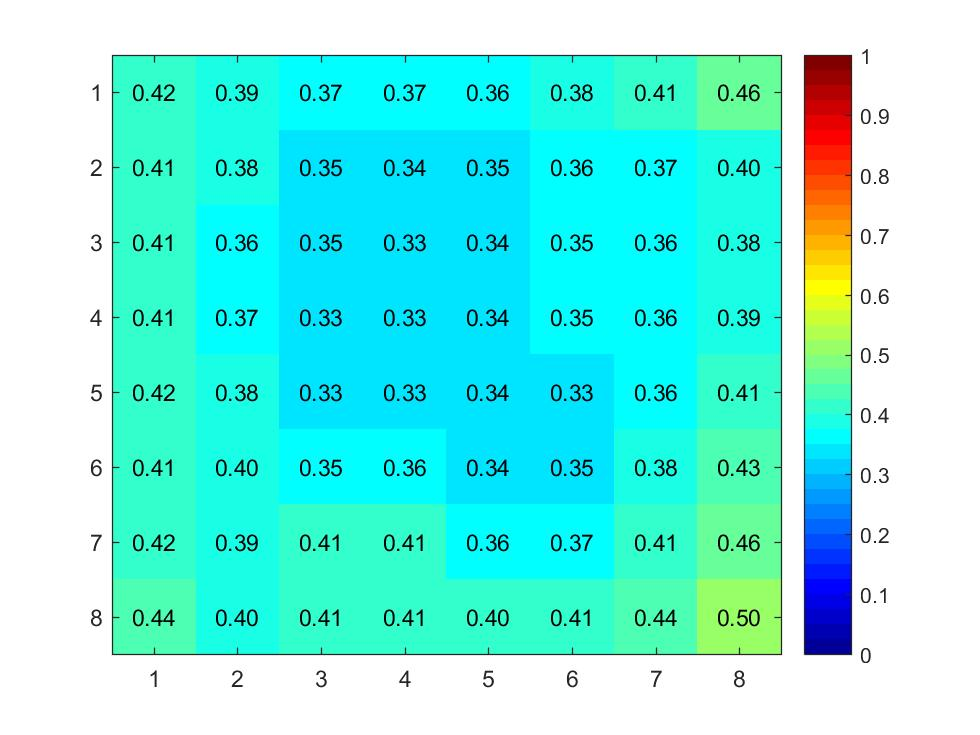
\includegraphics[width=0.5\textwidth]
	{fig/Distanz_140cm_std_.jpg}
	\caption[Streuung der einzelnen Pixel im Vergleich]{Streuung der einzelnen Pixel im Vergleich}
	\label{fig:Streuung}
\end{figure}


\section{Reflektion}




\section{Einfluss Störquellen}

Dieser Abschnitt befasst sich mit den Einfluss von externen Quellen auf den Sensor. Dabei spielen natürliche 



\section{Personenmessungen}
Bei der Personenmessungen wurden unterschiedliche Probanden in einem Aufzug ausgemessen auf dessen Wärmestrahlung.



\begin{figure}[H]
	\centering
	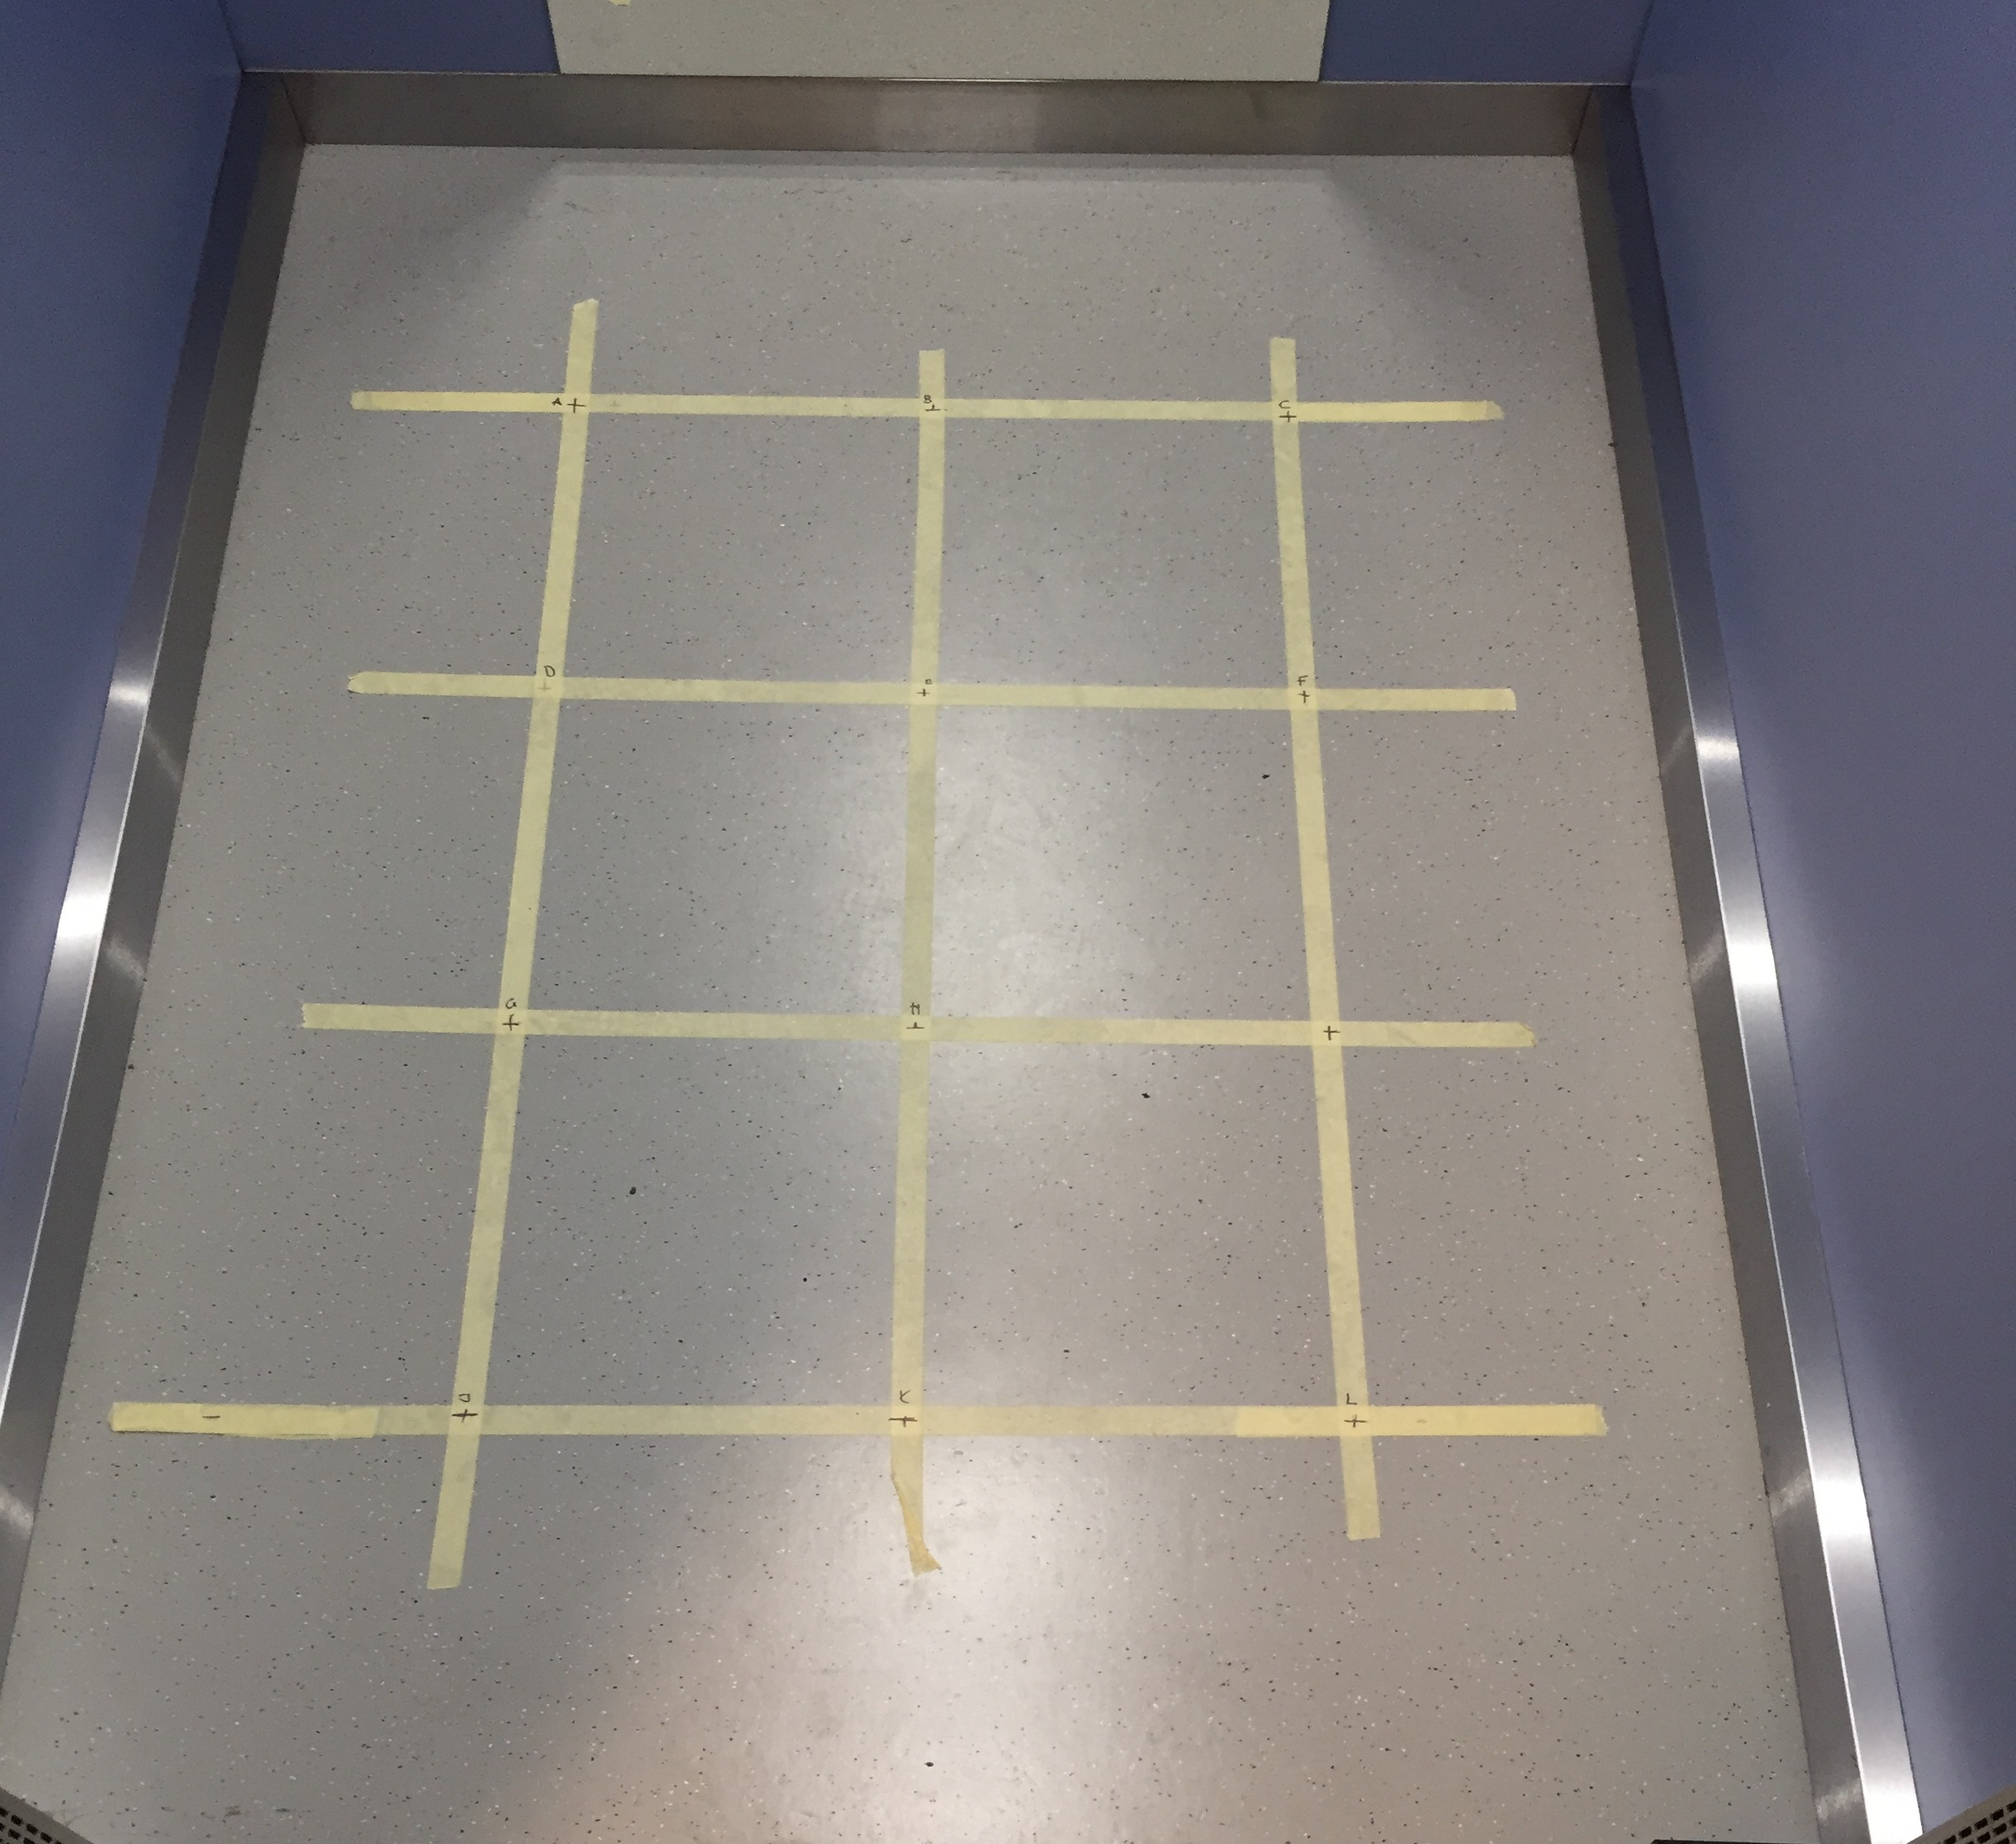
\includegraphics[width=0.8\textwidth, angle=270]
	{fig/Messraster.JPG}
	\caption[Personenmessung Messraster]{Personenmessung Messraster}
	\label{fig:Messraster}
\end{figure}













\section{Fazit}